% ----------------------------------------------------------------- %
%             The Speech Signal Processing Toolkit (SPTK)           %
%             developed by SPTK Working Group                       %
%             http://sp-tk.sourceforge.net/                         %
% ----------------------------------------------------------------- %
%                                                                   %
%  Copyright (c) 1984-2007  Tokyo Institute of Technology           %
%                           Interdisciplinary Graduate School of    %
%                           Science and Engineering                 %
%                                                                   %
%                1996-2016  Nagoya Institute of Technology          %
%                           Department of Computer Science          %
%                                                                   %
% All rights reserved.                                              %
%                                                                   %
% Redistribution and use in source and binary forms, with or        %
% without modification, are permitted provided that the following   %
% conditions are met:                                               %
%                                                                   %
% - Redistributions of source code must retain the above copyright  %
%   notice, this list of conditions and the following disclaimer.   %
% - Redistributions in binary form must reproduce the above         %
%   copyright notice, this list of conditions and the following     %
%   disclaimer in the documentation and/or other materials provided %
%   with the distribution.                                          %
% - Neither the name of the SPTK working group nor the names of its %
%   contributors may be used to endorse or promote products derived %
%   from this software without specific prior written permission.   %
%                                                                   %
% THIS SOFTWARE IS PROVIDED BY THE COPYRIGHT HOLDERS AND            %
% CONTRIBUTORS "AS IS" AND ANY EXPRESS OR IMPLIED WARRANTIES,       %
% INCLUDING, BUT NOT LIMITED TO, THE IMPLIED WARRANTIES OF          %
% MERCHANTABILITY AND FITNESS FOR A PARTICULAR PURPOSE ARE          %
% DISCLAIMED. IN NO EVENT SHALL THE COPYRIGHT OWNER OR CONTRIBUTORS %
% BE LIABLE FOR ANY DIRECT, INDIRECT, INCIDENTAL, SPECIAL,          %
% EXEMPLARY, OR CONSEQUENTIAL DAMAGES (INCLUDING, BUT NOT LIMITED   %
% TO, PROCUREMENT OF SUBSTITUTE GOODS OR SERVICES; LOSS OF USE,     %
% DATA, OR PROFITS; OR BUSINESS INTERRUPTION) HOWEVER CAUSED AND ON %
% ANY THEORY OF LIABILITY, WHETHER IN CONTRACT, STRICT LIABILITY,   %
% OR TORT (INCLUDING NEGLIGENCE OR OTHERWISE) ARISING IN ANY WAY    %
% OUT OF THE USE OF THIS SOFTWARE, EVEN IF ADVISED OF THE           %
% POSSIBILITY OF SUCH DAMAGE.                                       %
% ----------------------------------------------------------------- %
\hypertarget{fdrw}{}
\name{fdrw}{draw a graph}{plotting graphs}

\begin{synopsis}
\item[fdrw] [ --F $F$ ] [ --R $R$ ] [ --W $W$ ] [ --H $H$ ] [ --o $xo \; yo$ ] 
            [ --g $G$ ] [ --m $M$ ]   
\item[\ ~~~~~] [ --l $L$ ] [ --p $P$ ] [ --j $J$ ] [ --n $N$ ] [ --t $T$ ] 
	       [ --y $ymin \; ymax$ ] [ --z $Z$ ] [ --b ]  
\item[\ ~~~~~] [ {\em infile} ]
\end{synopsis}

\begin{qsection}{DESCRIPTION}
{\em fdrw} converts float data from {\em infile} (or standard input) 
to a plot formatted according to the FP5301 protocol, 
and sends the result to standard output.
One can control the details of the plot layout by setting the options bellow:
\end{qsection}

\begin{options}
	\argm{F}{F}{factor}{1}
	\argm{R}{R}{rotation angle}{0}
	\argm{W}{W}{width of figure ($\times 100$ mm)}{1}
	\argm{H}{H}{height of figure ($\times 100$ mm)}{1}
	\argm{o}{xo \; yo}{origin in mm}{20 25}
	\argm{g}{G}{draw grid ($0 \sim 2$)
                    (see also \hyperlink{fig}{fig})}{1}
	\argm{m}{M}{line type ($1 \sim 5$)\\
	\hspace*{2mm}1:~solid~~2:~dotted~~3:~dot and dash~~4:~broken~~5:~dash}{0}
	\argm{l}{L}{line pitch}{0}
	\argm{p}{P}{pen number ($1 \sim 10$)}{1}
	\argm{j}{J}{join number ($0 \sim 2$)}{1}
	\argm{n}{N}{number of samples}{0}
	\argm{t}{T}{rotation of coordinate axis. When $T=-1$, the
                    reference point is on the top-left. When $T=1$
                    the reference point is on the bottom-right.}{0}
	\argm{y}{ymin \; ymax}{scaling factor for $y$ axis}{-1 1}
	\argm{z}{Z}{This option is used when data is written
                    recursively in the $y$ axis. The distance between
                    two graphs in the $y$ axis is given by $Z$.}{0}
	\argm{b}{}{bar graph mode}{FALSE}
	\desc[1ex]{The $x$ axis scaling is automatically done so that
                every point in the input file is plotted in equally
                spaced  interrals
                for the assigned width.
                When the {\bf --n} option is omitted and the number of
                input samples is below 1000000, then the block size is made
                equal to the number of samples.
                When the number of samples is above 1000000,
                then the block size is made equal to 1000000.}
	\desc{When the {\bf --y} option is omitted,
		the input data minimum value is set to $ymin$
                and the maximum value is set to $ymax$.}
\end{options}

\begin{qsection}{EXAMPLE}
In the example below, the impulse response of a digital filter is
drawn on the X window environment:
\begin{quote}
  \verb!impulse | dfs -a 1 0.8 0.5 | fdrw -W 1.0 -H 0.3 | xgr!
\end{quote}
\begin{center}
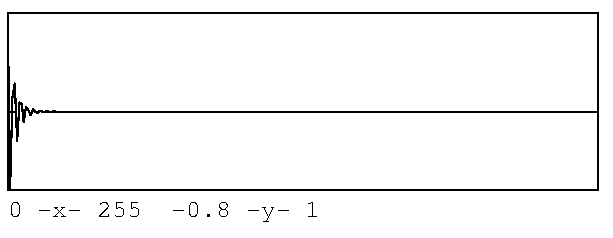
\includegraphics[width=6cm]{fig/fdrw_1.pdf}
\end{center}

The graph width is 10cm and its height is 3cm.
\par
The next example draws the magnitude of
the frequency response of a digital filter on the X window environment:
\begin{quote}
  \verb!impulse | dfs -a 1 0.8 0.5 | spec | fdrw -y -60 40 | xgr!
\end{quote}
\begin{center}
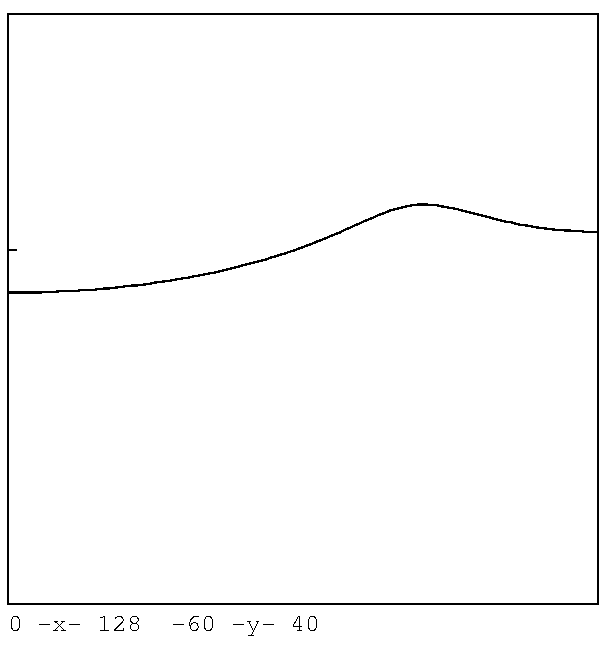
\includegraphics[width=6cm]{fig/fdrw_2.pdf}
\end{center}

The $y$ axis goes from $-60$ dB to $40$ dB.
\par
The running spectrum can be draw on the X window environment by:
\begin{quote}
 \verb!fig -g 0 -W 0.4 << EOF ; ! \\
 \verb!~~~~x 0 5 !\\
 \verb!~~~~xscale 0 1 2 3 4 5 !\\
 \verb!~~~~xname "FREQUENCY (kHz)"!\\
 \verb!EOF!\\
 \verb!spec < data |\ !\\
 \verb!fdrw -W 0.4 -H 0.2 -g 0 -n 257 -y -40 40 -z 1.7 |\ !\\
 \verb!xgr !
\end{quote}
\begin{center}
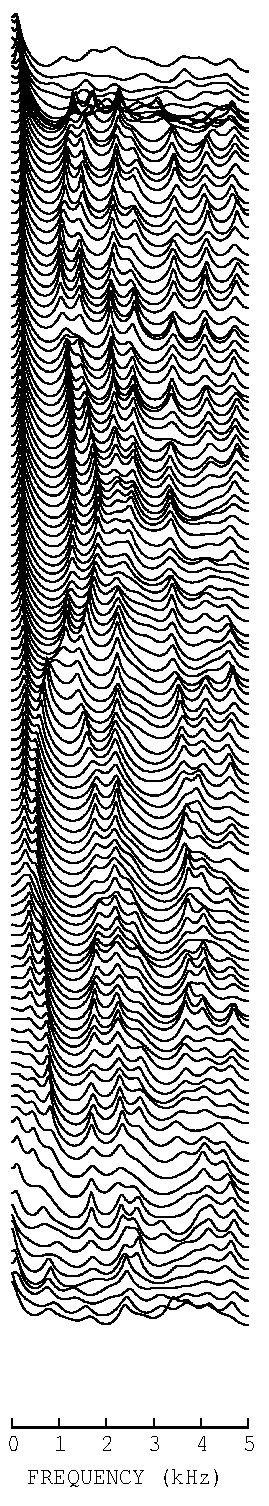
\includegraphics[width=3cm]{fig/fdrw_3.pdf}
\end{center}

The command {\em psgr} prints the output to a laser printer in the
same manner as it is printed on the screen.
Since the {\em fdrw} command includes a sequence of commands
for a plotter machine (FP5301 protocol) in the output file,
its output can be directly sent to a printer.
\end{qsection}

\begin{qsection}{SEE ALSO}
\hyperlink{fig}{fig},
\hyperlink{xgr}{xgr},
\hyperlink{psgr}{psgr}
\end{qsection}
